% =============================================================================
% Module 18: The Mass-Sheet Degeneracy in Multi-Plane Lenses and Kinematic Breaking
% =============================================================================
% Part V — Compound Lenses, Degeneracies, and Cosmography
% Sources: Falco, Gorenstein & Shapiro (1985); Schneider (2014, A&A 568, L2);
%          Schneider (2019, A&A 624, A54); Schneider & Sluse (2013, 2014);
%          Congdon & Keeton Sect. 4.7.2; Meneghetti Sect. 5.9;
%          Saha et al. (2024) Sect. 3.7; Birrer et al. (2020)
% Mathematica: ../Mathematica/18_MSD_Kinematics/msd_multiplane.wl
% Solutions:   ../Solutions/18_MSD_Kinematics/problems_18.wl
% =============================================================================

\chapter{The Mass-Sheet Degeneracy in Multi-Plane Lenses and Kinematic Breaking}
\label{ch:msd_kinematics}

\noindent
Chapter~\ref{ch:galaxy_lensing} introduced the mass-sheet transformation
(MST), $\kappab\to\lambda\kappab+(1-\lambda)$, proved that it leaves image
positions and flux ratios untouched (\S\ref{sec:msd}), placed it inside the
wider family of source-position transformations (\S\ref{sec:spt}), and showed
that it propagates one-for-one into a time-delay Hubble constant
(Eq.~\ref{eq:mst_H0}).  Chapter~\ref{ch:weak_lensing} met the same
transformation as the reason a shear map determines $\kappab$ only up to a
constant (\S\ref{sec:wl_reduced_shear}).  This chapter asks the two questions
that matter once lenses have more than one source plane, and once one wants to
\emph{do} something about the degeneracy:
\begin{enumerate}[nosep]
    \item Does a second source plane behind the same deflector break the MST?
          (Answer: only if the distance ratio between the planes is known in
          advance --- which, in double-source-plane cosmography, is exactly
          what one is trying to measure.)
    \item How does a stellar velocity dispersion fix $\lambda$, and which
          systematic errors does it bring with it?
\end{enumerate}
Along the way we show that a change of the power-law slope $\gp$ is, to first
order near the Einstein radius, an MST in disguise.  That ``local MST'' is the
mechanism through which an unmodelled central mass biases both a time-delay
$\Hubble$ and a double-source-plane distance ratio
(Chapter~\ref{ch:central_mass_bias}).

\medskip
\noindent
\textbf{Companion Mathematica files:}
\begin{itemize}[nosep]
    \item \mathlink{18_MSD_Kinematics/msd_multiplane.wl}{msd\_multiplane.wl}
          --- symbolic verification of every result in this chapter: the
          single-plane MST (SIS and power law $+$ sheet), the two-source-plane
          and two-lens-plane transformations, the local MST, and the spherical
          Jeans solution for a power-law lens; exports
          Fig.~\ref{fig:ms_powerlaw_kappa}
    \item \solnlink{18_MSD_Kinematics/problems\_18.wl}{problems\_18.wl}
          --- worked solutions to the problems of \S\ref{sec:ms_problems}
\end{itemize}


% =====================================================================
\section{The Mass-Sheet Transformation in Three Lines}
\label{sec:ms_three_lines}

Let $\kappab(\vectheta)$ be any lens that reproduces a set of images.  The
MST (\citealp{falco_gorenstein_shapiro_1985}; Eq.~\ref{eq:mst_kappa})
replaces it by
\begin{equation}
    \kappab_\lambda(\vectheta) = \lambda\,\kappab(\vectheta) + (1-\lambda),
    \qquad \lambda\neq0 .
    \label{eq:ms_mst}
\end{equation}
Three facts carry the whole argument.  (i) The deflection is linear in
$\kappab$, and a uniform sheet $\kappab=1$ deflects as
$\vecalpha_{\rm sheet}=\vectheta$ (for an axisymmetric distribution
$\alpha=\bar\kappab\,\theta$, Eq.~\ref{eq:alpha_mean_kappa}, and here
$\bar\kappab=1$).  Hence
\begin{equation}
    \vecalpha_\lambda(\vectheta)=\lambda\,\vecalpha(\vectheta)+(1-\lambda)\,\vectheta .
    \label{eq:ms_alpha}
\end{equation}
(ii) Inserting this into the lens equation,
\begin{equation}
    \boxed{\;
    \vectheta-\vecalpha_\lambda(\vectheta)
    =\vectheta-\lambda\vecalpha-(1-\lambda)\vectheta
    =\lambda\,\bigl[\vectheta-\vecalpha(\vectheta)\bigr]
    =\lambda\,\vecbeta ,\;}
    \label{eq:ms_three_lines}
\end{equation}
so every $\vectheta$ that solved the original lens equation for a source at
$\vecbeta$ solves the transformed one for a source at $\lambda\vecbeta$
\annot{check s1 of \texttt{msd\_multiplane.wl}}.
(iii) Differentiating Eq.~\eqref{eq:ms_alpha} gives
$\Amat_\lambda=\lambda\Amat$ (Eq.~\ref{eq:mst_jacobian}), and the Fermat
potential (Eq.~\ref{eq:fermat_potential}) transforms as
\begin{equation}
    \tau_\lambda(\vectheta)=\tfrac12|\vectheta-\lambda\vecbeta|^2
      -\lambda\psiL(\vectheta)-\tfrac{1-\lambda}{2}|\vectheta|^2
    =\lambda\,\tau(\vectheta)+\tfrac{\lambda(\lambda-1)}{2}|\vecbeta|^2 .
    \label{eq:ms_fermat}
\end{equation}
The last term is the same for every image, so it cancels from any difference:
$\Delta\tau_\lambda=\lambda\,\Delta\tau$.

\begin{derivation}[The Fermat potential under the MST]
Write $\psiL_\lambda=\lambda\psiL+\tfrac{1-\lambda}{2}|\vectheta|^2$; its
Laplacian is $2\lambda\kappab+2(1-\lambda)=2\kappab_\lambda$, as it must be.
Expand the geometric term with the rescaled source,
$\tfrac12|\vectheta-\lambda\vecbeta|^2
=\tfrac12|\vectheta|^2-\lambda\,\vectheta\cdot\vecbeta+\tfrac{\lambda^2}{2}|\vecbeta|^2$,
and subtract $\psiL_\lambda$:
\[
\tau_\lambda=\tfrac{\lambda}{2}|\vectheta|^2-\lambda\,\vectheta\cdot\vecbeta
+\tfrac{\lambda^2}{2}|\vecbeta|^2-\lambda\psiL .
\]
Compare with
$\lambda\tau=\tfrac{\lambda}{2}|\vectheta|^2-\lambda\,\vectheta\cdot\vecbeta
+\tfrac{\lambda}{2}|\vecbeta|^2-\lambda\psiL$.
The difference is $\tfrac{\lambda^2-\lambda}{2}|\vecbeta|^2$, independent of
$\vectheta$ \annot{checks s12--s13}.
\end{derivation}

\begin{keybox}[What the MST preserves and what it changes]
Under Eq.~\eqref{eq:ms_mst} with $\vecbeta\to\lambda\vecbeta$:
\begin{itemize}[nosep,leftmargin=1.2em]
    \item \textbf{Unchanged:} image positions; image shapes ($\Amat_\lambda\propto\Amat$);
          flux ratios; critical curves (both eigenvalues $1-\kappab\pm\gammaL$
          scale by $\lambda$, so their zeros stay put); the Einstein radius
          (where $\bar\kappab_\lambda=\lambda\bar\kappab+1-\lambda=1$ iff
          $\bar\kappab=1$); the reduced shear.
    \item \textbf{Changed:} absolute magnifications $\mu\to\mu/\lambda^2$;
          time delays $\Delta t\to\lambda\,\Delta t$, hence
          $\Hubble^{\rm true}=\lambda\,\Hubble^{\rm naive}$
          (Eq.~\ref{eq:mst_H0}); the mass of the deflector itself.
\end{itemize}
\annot{checks s6--s14}
\end{keybox}

\begin{bridge}[Magnification, time delays, and galaxy lensing]
Every line above is a re-use.  $\Amat=\mathbb{I}-\nabla\nabla\psiL$ and its
eigenvalues $1-\kappab\pm|\gammaL|$ are Eq.~\eqref{eq:eigenvalues} of
Chapter~\ref{ch:magnification}; the Fermat potential and the factor that turns
$\Delta\tau$ into $\Delta t$ are
Eqs.~\eqref{eq:fermat_potential}--\eqref{eq:t_tau_relation} of
Chapter~\ref{ch:fermat_time_delays}; the componentwise proof of
$\Amat_\lambda=\lambda\Amat$ and the $\Hubble$ bookkeeping are in
\S\ref{sec:msd} of Chapter~\ref{ch:galaxy_lensing}.  The same transformation
appears as Congdon \& Keeton's Eq.~(4.88) \citep{congdon_principles_2018},
Meneghetti's Eqs.~(5.146)--(5.150) \citep{meneghetti_introduction_2021}, and
Eq.~(51) of \citet{saha_essentials_2024}, where it is also called the
\emph{steepness degeneracy}.
\end{bridge}

\begin{annotation}[Which way does $\Hubble$ go?]
The relation $\Delta t\to\lambda\Delta t$ is a statement about \emph{models}
at fixed $\Hubble$.  Data run the other way: the observed delay is fixed, so
a model whose $\Delta\tau$ is larger by $\lambda$ needs a time-delay distance
smaller by $\lambda$, i.e.\ an $\Hubble$ larger by $\lambda$.  If the truth
contains a sheet ($\lambda<1$, a positive sheet) and one fits without it, the
fit returns $\Hubble^{\rm naive}=\Hubble^{\rm true}/\lambda$, too high.
Write it once as Eq.~\eqref{eq:mst_H0} and never re-derive the direction
from memory: the direction is easy to get backwards \annot{check s14}.
\end{annotation}

\subsection{Two explicit examples}
\label{sec:ms_examples}

It is worth seeing Eq.~\eqref{eq:ms_three_lines} work on actual profiles.
For an SIS (Chapter~\ref{ch:axisymmetric_models}), on the axis through the
source, $\alpha(\theta)=\thetaE\,{\rm sgn}(\theta)$ and the images of a source
at $0<\beta<\thetaE$ sit at $\theta_\pm=\beta\pm\thetaE$.  With a sheet,
$\theta-\alpha_\lambda=\lambda(\theta-\thetaE\,{\rm sgn}\,\theta)$, which equals
$\lambda\beta$ at exactly the same $\theta_\pm$ \annot{check s3}.  For a power law
(Eq.~\ref{eq:kappa_power_law}),
\begin{equation}
    \kappab(\theta)=\frac{3-\gp}{2}\Bigl(\frac{\thetaE}{\theta}\Bigr)^{\gp-1},
    \qquad
    \alpha(\theta)=\thetaE\,{\rm sgn}(\theta)\Bigl(\frac{|\theta|}{\thetaE}\Bigr)^{2-\gp},
    \label{eq:ms_powerlaw}
\end{equation}
the identity $\theta-\alpha_\lambda(\theta)-\lambda\beta=\lambda[\theta-\alpha(\theta)-\beta]$
holds for every $\theta$ \annot{check s4}, so the roots are shared; for
$\gp=2.2$ and $\beta=0.2\,\thetaE$ they are $\theta_A=1.1692\,\thetaE$ and
$\theta_B=-0.8364\,\thetaE$ for every $\lambda$ \annot{check s5}.
Figure~\ref{fig:ms_powerlaw_kappa} shows three such profiles and the shared roots.

\begin{figure}[ht]
    \centering
    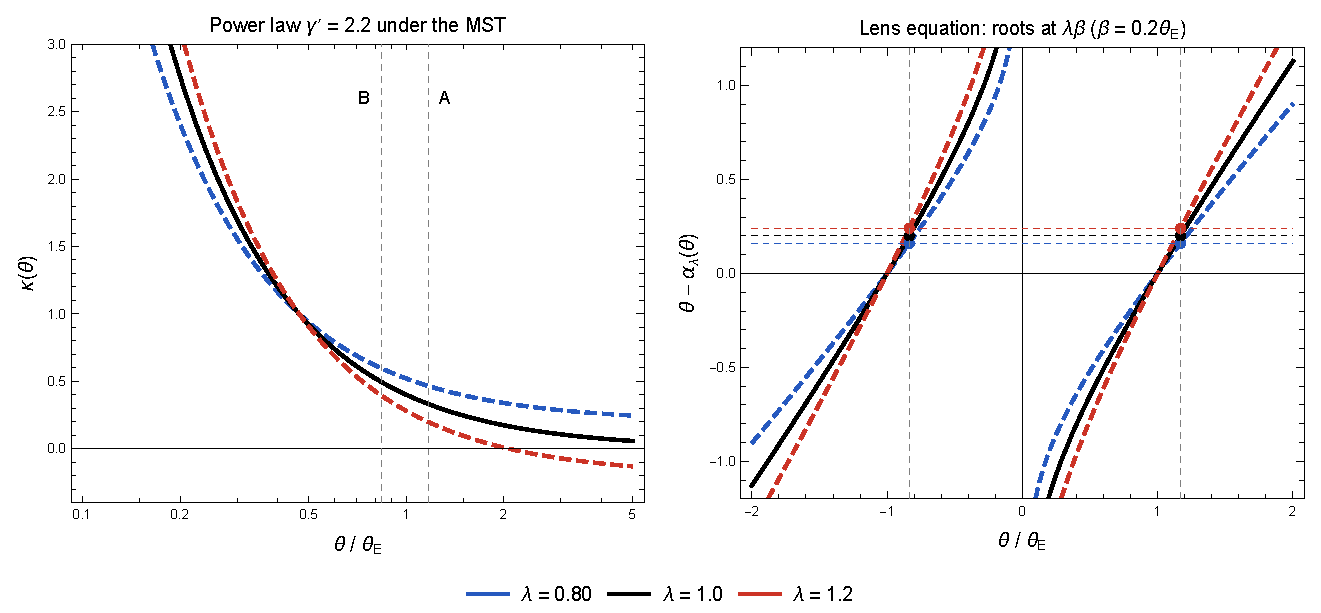
\includegraphics[width=\textwidth]{../Figures/18_MSD_Kinematics/msd_powerlaw_kappa.pdf}
    \caption{The MST of a power law with $\gp=2.2$.  \textbf{Left:} convergence
    for $\lambda=0.8$ (positive sheet), $1$, and $1.2$ (negative sheet; this
    profile crosses $\kappab=0$ near $2\,\thetaE$).  All three profiles
    cross where $\kappab=1$ (the fixed point of $\kappab\to\lambda\kappab+1-\lambda$),
    not at $\thetaE$.  The dashed verticals mark the two images A and B of a
    source at $\beta=0.2\,\thetaE$; they are the same for all three profiles.
    \textbf{Right:} the lens map $\theta-\alpha_\lambda(\theta)$.  Each curve
    meets its own source line $\lambda\beta$ (horizontal dashes) at the same
    two image positions.  Generated by \texttt{msd\_multiplane.wl}.}
    \label{fig:ms_powerlaw_kappa}
\end{figure}

\begin{annotation}[Reading the figure]
A positive sheet ($\lambda<1$) makes the profile \emph{shallower}: it lowers
$\kappab$ inside the $\kappab=1$ crossing and raises it outside.  A negative
sheet steepens it.  This is the ``steepness'' in Saha et al.'s name for the
degeneracy, and it previews \S\ref{sec:ms_local}: near the images, adding a
sheet looks like changing $\gp$.  Note also that the $\lambda=1.2$ profile
goes negative at large radius.  A global MST with $\lambda>1$ is unphysical,
but only the region the images probe has to be reproduced.
\end{annotation}


% =====================================================================
\section{What the Sheet Is: External, Internal, and the SPT}
\label{sec:ms_what_sheet}

The parameter $\lambda$ has two physically different readings, and different
data break them.
\begin{itemize}
    \item \textbf{External sheet.}  Line-of-sight structure adds a nearly
          uniform convergence $\kappa_{\rm ext}$ across the image region; it is
          an MST with $\lambda=1-\kappa_{\rm ext}$
          (\S\ref{sec:external_convergence}, Eq.~\ref{eq:kappa_ext_H0}).  The
          deflector's own mass is untouched; the sheet is real matter
          elsewhere, estimated from galaxy counts and weak lensing of the
          field rather than from the lens.
    \item \textbf{Internal sheet.}  No extra matter exists; instead the
          deflector's own profile is $\lambda\kappab+(1-\lambda)\kappab_{\rm c}$,
          where $\kappab_{\rm c}$ is a very extended, cored component that is
          nearly constant over the image region.  This is a re-profiling of the
          galaxy that imaging cannot see, and field counts cannot touch it.
          \citet{schneider_sluse_2013} argue that the formal precision of
          time-delay $\Hubble$ rests on assuming that the profile is an exact
          power law, which suppresses exactly this freedom.
\end{itemize}
The MST is itself the exactly-degenerate, profile-independent member of the
\emph{source-position transformations} (SPT;
\citealp{schneider_sluse_2014}; \S\ref{sec:spt}), which remap the source plane
non-linearly and keep the images invariant only approximately.  Everything in
this chapter concerns the exact, linear member.

\begin{bridge}[Weak lensing and the sheet]
In Chapter~\ref{ch:weak_lensing} the same transformation,
Eq.~\eqref{eq:wl_mst}, leaves the reduced shear $g=\gammaL/(1-\kappab)$
invariant (Eq.~\ref{eq:wl_g_invariant}); a shear map therefore fixes $\kappab$
only up to the constant $\kappab_0$ of the Kaiser--Squires inversion.  A
weak-lensing estimate of $\kappa_{\rm ext}$ around a strong lens inherits that
freedom and has to be anchored separately, for example by number counts or by
assuming $\kappab\to0$ far from the lens.
\end{bridge}


% =====================================================================
\section{One Deflector, Two Source Planes}
\label{sec:ms_two_sources}

Now place two sources behind the same deflector at redshift $z_d$: a nearer one
(plane~1, $z_{s1}$) and a farther one (plane~2, $z_{s2}>z_{s1}$).  For the
moment the nearer source is massless, so a single plane deflects both.  The
deflector has one physical surface density $\Sigma(\vectheta)$ but two
convergences,
\begin{equation}
    \kappab_i(\vectheta)=\frac{\Sigma(\vectheta)}{\Sigma_{{\rm cr},i}},
    \qquad
    \kappab_1=\Brat\,\kappab_2,
    \qquad
    \Brat\equiv\frac{\Sigma_{{\rm cr},2}}{\Sigma_{{\rm cr},1}}
     =\frac{\Dls{d}{s1}\,\Dls{}{s2}}{\Dls{}{s1}\,\Dls{d}{s2}}<1 ,
    \label{eq:ms_brat}
\end{equation}
with $\Sigma_{{\rm cr},i}=c^2\Dls{}{si}/(4\pi G\Dd\Dls{d}{si})$
(Eq.~\ref{eq:sigma_cr_recap}).  The ratio $\Brat$ depends only on redshifts
and on the expansion history; measuring it is the point of
double-source-plane (DSPL) cosmography (Chapter~\ref{ch:multiplane_dspl};
\citealp{collett_2012,collett_auger_2014}).  Its observable proxy is the ratio
of the two Einstein radii,
\begin{equation}
    \etamea\equiv\frac{\theta_{\rm E1}}{\theta_{\rm E2}},
    \qquad
    \Brat=\etamea^{\,\gp-1}\quad\text{(power law)},
    \label{eq:ms_eta}
\end{equation}
which follows from $\bar\kappab_2(\theta)=(\theta_{\rm E2}/\theta)^{\gp-1}$
\annot{check s11} and $\bar\kappab_1=\Brat\,\bar\kappab_2=1$ at $\theta_{\rm E1}$.
Throughout this chapter plane~1 is the \emph{nearer} source, so that
$\Brat<1$ and $\etamea<1$; $\etamea$ always denotes the ratio of Einstein radii
and $\Brat$ the distance ratio (papers that number the planes the other way
quote $\Brat^{-1}$).

\begin{bridge}[Distances and critical densities]
$\Brat$ is the ratio of the two lensing distance ratios
$\mathcal{D}\equiv\Dds/(\Dd\Ds)$ of Chapter~\ref{ch:cosmological_distances}
(\S\ref{sec:distance_ratio}, Eq.~\ref{eq:distance_ratio}), one per source;
the common $\Dd$ cancels, leaving $\Brat=(\Dls{d}{s1}/\Dls{}{s1})/(\Dls{d}{s2}/\Dls{}{s2})$.  The prefactor $c/\Hubble$
cancels, which is why a DSPL measures the shape of $D(z)$, and hence
$\Omega_{\rm m}$ and $w$, but not $\Hubble$.
\end{bridge}

\subsection{Known distances: the second plane breaks the MST}
\label{sec:ms_known}

Suppose $\Brat$ is known.  Is there still an MST?  Transform the physical
density as $\Sigma\to\lambda_m\Sigma+\Sigma_s$.  Plane by plane,
$\kappab_i\to\lambda_m\kappab_i+\Sigma_s/\Sigma_{{\rm cr},i}$, and this is an
MST of plane $i$ only if $\Sigma_s/\Sigma_{{\rm cr},i}=1-\lambda_m$.  Both
conditions can hold only if $\lambda_m=1$ and $\Sigma_s=0$, because
$\Sigma_{{\rm cr},1}\neq\Sigma_{{\rm cr},2}$ \annot{check t1}.  Concretely, apply an
MST $\lambda_2$ to the far plane.  The near plane then receives
\begin{equation}
    \kappab_1'=\lambda_2\,\kappab_1+\Brat\,(1-\lambda_2),
    \qquad
    \vectheta-\vecalpha_1'=\bigl[1-\Brat(1-\lambda_2)\bigr]\vectheta-\lambda_2\vecalpha_1 ,
    \label{eq:ms_known}
\end{equation}
which is not proportional to $\vectheta-\vecalpha_1$ unless $\lambda_2=1$
\annot{checks t2a--t2b}: the near-plane images move.  For the power law the near
Einstein radius shifts to
\begin{equation}
    \Bigl(\frac{\theta_{\rm E1}'}{\theta_{\rm E1}}\Bigr)^{\gp-1}
    =\frac{\lambda_2}{1-\Brat(1-\lambda_2)} ,
    \label{eq:ms_thetaE1_shift}
\end{equation}
so for $\gp=2$, $\Brat=0.7$, $\lambda_2=0.9$, $\etamea$ falls by $3.2\%$
\annot{checks t2c--t2d}.  This is the sense in which ``multiple source planes break
the MSD'' (\S\ref{sec:msd}, item~3; \citealp{saha_essentials_2024}, \S3.7):
the sheet is one physical object, and its convergence scales as
$1/\Sigma_{{\rm cr},i}$, differently on each plane.

\subsection{Free distance ratio: the second plane does not}
\label{sec:ms_free}

In DSPL cosmography $\Brat$ is \emph{not} known; it is the measurement.  So let
the model carry its own ratio $\Brat'$ and ask whether a pair of per-plane MSTs
$(\lambda_1,\lambda_2)$ can reproduce both image sets.  The far plane is
transformed with $\lambda_2$, and the model's near-plane convergence is
$\Brat'$ times the transformed far-plane one.  Demanding that this be an exact
MST of the true near plane,
$\Brat'\bigl[\lambda_2\kappab_2+1-\lambda_2\bigr]
=\lambda_1\Brat\kappab_2+(1-\lambda_1)$ for every $\kappab_2$, gives two
linear conditions with the unique solution
\begin{equation}
    \boxed{\;
    \Brat'=\frac{1}{1-\lambda_2+\lambda_2/\Brat},
    \qquad
    \lambda_1=\frac{\lambda_2}{\Brat(1-\lambda_2)+\lambda_2},
    \qquad
    \frac{1-\lambda_1}{1-\lambda_2}=\Brat' .\;}
    \label{eq:ms_free}
\end{equation}

\begin{derivation}[Solving for $\Brat'$ and $\lambda_1$]
Match the coefficient of $\kappab_2$: $\Brat'\lambda_2=\lambda_1\Brat$.  Match
the constant: $\Brat'(1-\lambda_2)=1-\lambda_1$.  Substitute
$\lambda_1=\Brat'\lambda_2/\Brat$ into the second:
$\Brat'(1-\lambda_2)=1-\Brat'\lambda_2/\Brat$, i.e.\
$\Brat'\bigl[1-\lambda_2+\lambda_2/\Brat\bigr]=1$.  Then
$\lambda_1=\lambda_2\Brat'/\Brat=\lambda_2/\bigl[\Brat(1-\lambda_2)+\lambda_2\bigr]$.
The last identity in Eq.~\eqref{eq:ms_free} is the constant-term condition
rewritten \annot{checks t3a--t3c, t3i}.
\end{derivation}

Three features of Eq.~\eqref{eq:ms_free} carry the physics.
\begin{itemize}
    \item The two planes carry \emph{different} mass-sheet parameters:
          $\lambda_1-\lambda_2=\lambda_2(1-\lambda_2)(1-\Brat)/[\Brat(1-\lambda_2)+\lambda_2]$,
          non-zero unless $\lambda_2=1$ \annot{check t3d}.
    \item The two sheets are one physical sheet at the deflector:
          $(1-\lambda_1)/(1-\lambda_2)=\Brat'$ is exactly the ratio that a
          uniform $\Sigma_s$ at $z_d$ produces between the two planes, read
          through the model's distance ratio.  The $\lambda_i$ differ
          \emph{because} the sheet sits physically at the lens plane.
    \item Each plane's Einstein radius is fixed by its own exact MST, so both
          $\theta_{{\rm E}i}$ and $\etamea$ are unchanged \annot{check t3e}, while
          the inferred distance ratio moves.  For $\Brat=0.7$, $\lambda_2=0.9$:
          $\Brat'=70/97=0.7216$ and $\lambda_1=90/97=0.9278$ \annot{check t3f}.  To
          first order,
          \begin{equation}
              \Brat'\simeq\Brat\,\bigl[1+(1-\Brat)(1-\lambda_2)\bigr],
              \label{eq:ms_free_linear}
          \end{equation}
          so a positive sheet ($\lambda_2<1$) is mistaken for a larger
          distance ratio \annot{check t3g}.
\end{itemize}

\begin{keybox}[A second source plane trades $\lambda$ for $\Brat$]
For a single deflector with sources on two planes, a mass sheet at the lens
redshift acts on each plane as an exact MST with its own $\lambda_i$, provided
the distance ratio is allowed to change according to Eq.~\eqref{eq:ms_free}.
All images on both planes and the Einstein-radius ratio $\etamea$ are
invariant.  If $\Brat$ is known (cosmology fixed), the second plane breaks the
MST; if $\Brat$ is the target, the MST and the cosmology are degenerate, and an
independent handle on $\lambda$ is required.
\end{keybox}

\begin{annotation}[The argument in words]
A sheet is a magnifying glass of fixed strength placed at the lens.  Seen from
the far source it has convergence $1-\lambda_2$; seen from the near source,
which sits closer behind the glass, the same glass is weaker.  If you know the
geometry, the mismatch between the two planes exposes the glass.  If the
geometry (the distance ratio) is what you are fitting, you can always choose a
geometry in which the weaker near-plane sheet is exactly what an MST of the
near plane requires, and nothing in either set of images objects.  A second
source plane gives you a second ruler, but both rulers are read through the
same unknown lens.
\end{annotation}

\subsection{How the MST reaches a power-law distance ratio}
\label{sec:ms_pl_reading}

With a power-law model, $\Brat=\etamea^{\,\gp-1}$ contains no mass
normalisation at all: $\partial\Brat/\partial\lambda=0$ at fixed $(\etamea,\gp)$,
whereas $\partial\Brat/\partial\gp=\Brat\ln\etamea\neq0$ \annot{check t3h}.  Since
$\etamea$ is invariant, a power-law fit can follow the shift
$\Brat\to\Brat'$ of Eq.~\eqref{eq:ms_free} only by changing its slope,
$\gp'-1=(\gp-1)\ln\Brat'/\ln\Brat$.  For the DSPL ratio the MST is therefore
demoted from a normalisation systematic (as it is for $\Hubble$) to a
\emph{profile-shape} systematic.  Anything that drags the fitted $\gp$ --- a
sheet, a core, a central point mass --- moves $\Brat$ by
$\delta\ln\Brat=\ln\etamea\,\delta\gp$.  Section~\ref{sec:ms_local} makes the
link between ``sheet'' and ``slope'' precise.

\subsection{When the nearer source has mass: two lens planes}
\label{sec:ms_two_lens}

In many DSPLs the first source is itself a galaxy massive enough to deflect
light from the second.  \citet{schneider_2014_multiplane} showed that the MST
survives this too.  With $\vectheta$ the image-plane position, $\Brat$ his
$\beta$, and deflections scaled to the last plane, the lens equations are
\begin{equation}
    \vectheta_2=\vectheta-\Brat\,\vecalpha_1(\vectheta),
    \qquad
    \vectheta_3=\vectheta-\vecalpha_1(\vectheta)-\vecalpha_2(\vectheta_2),
    \label{eq:ms_twoplane}
\end{equation}
and the transformation
\begin{equation}
    \vecalpha_1'=\lambda\vecalpha_1+\frac{1-\lambda}{\Brat}\vectheta,
    \qquad
    \vecalpha_2'(\vectheta_2')=\vecalpha_2(\vectheta_2'/\lambda)
       +\frac{\lambda-1}{\lambda\Brat}\,\vectheta_2'
    \label{eq:ms_schneider}
\end{equation}
gives $\vectheta_2'=\lambda\vectheta_2$ and $\vectheta_3'=\vectheta_3$
(\citealp{schneider_2014_multiplane}, Eqs.~6--11; checks t4a--t4b).

\begin{derivation}[Why the far plane is not rescaled]
Ansatz: $\vecalpha_2'(\vectheta_2')=\nu_3\vecalpha_2(\vectheta_2'/\lambda)+K_2\vectheta_2'$
with $\vectheta_2'=\lambda(\vectheta-\Brat\vecalpha_1)$.  Then
\[
\vectheta_3'=\vectheta-\lambda\vecalpha_1-\tfrac{1-\lambda}{\Brat}\vectheta
-\nu_3\vecalpha_2-K_2\lambda\vectheta+K_2\lambda\Brat\vecalpha_1 .
\]
Require $\vectheta_3'=\nu_3\vectheta_3=\nu_3(\vectheta-\vecalpha_1-\vecalpha_2)$.
The $\vecalpha_2$ terms agree by construction.  The $\vecalpha_1$ terms give
$\lambda-K_2\lambda\Brat=\nu_3$; the $\vectheta$ terms give
$1-(1-\lambda)/\Brat-K_2\lambda=\nu_3$.  From the first,
$K_2\lambda=(\lambda-\nu_3)/\Brat$; inserting this into the second and
multiplying by $\Brat$ gives $\Brat-1+\nu_3=\Brat\nu_3$, i.e.\
$(\Brat-1)(1-\nu_3)=0$.  Since $\Brat<1$, $\nu_3=1$ and
$K_2=(\lambda-1)/(\lambda\Brat)$.  Check t4b solves the same linear system.
\end{derivation}

Three consequences follow.  (i) The sheets alternate in sign: plane~1 receives
$K_1=(1-\lambda)/\Brat$ and plane~2 receives $K_2=(\lambda-1)/(\lambda\Brat)$,
with $K_1/K_2=-\lambda$ \annot{check t4c; Problem~\ref{ex:ms_schneider}}.  (ii) The
second lens is rescaled in amplitude and in scale:
$\vecalpha_2(\vectheta_2'/\lambda)$ is the deflection of
$\lambda^{-1}\kappab_2(\vectheta/\lambda)$ (Schneider's Eq.~13; check t4d for a
power law).  (iii) All time delays, from sources on both planes, scale by the
same $\lambda$, so time-delay \emph{ratios} cannot break the transformation
\citep{schneider_2014_multiplane}.  The same paper shows that a change of
cosmology, $\Brat\to\Brat'$, can be absorbed by a transformation of the same
form (his Eqs.~18--20; checks t4e--t4f2); with the first source made massless
this reduces to our Eq.~\eqref{eq:ms_free} \annot{check t4g}.  For an arbitrary
number of planes the isotropic scaling alternates between $\lambda$ and $1$
from plane to plane, and every time delay still scales by $\lambda$
\citep{schneider_2019_generalized}.

\begin{annotation}[Common error]
Do not conclude from $\nu_3=1$ that the far plane is unaffected.  Its image
positions are unchanged, as they must be, and its source plane is not
rescaled; but the mass in plane~2 has been rescaled and a negative sheet has
been added.  A standard candle on the far source plane would not detect the
MST; one on the near source plane would, since its magnifications scale by
$\lambda^{-2}$.
\end{annotation}


% =====================================================================
\section{The Power-Law Slope as a Local MST}
\label{sec:ms_local}

Strong lensing probes $\kappab$ only in an annulus around $\thetaE$, so the
transformation need only hold there; its main effect is to change the local
slope of the profile near the Einstein radius \citep{schneider_2014_multiplane}.
To see how, expand the deflection of a power law and of its MST about
$\theta=\thetaE+\delta$ ($\theta>0$):
\begin{align}
    \alpha_{\gp}(\thetaE+\delta) &= \thetaE+(2-\gp)\,\delta
      +\frac{(2-\gp)(1-\gp)}{2\thetaE}\,\delta^2+\order{\delta^3},
    \label{eq:ms_local_pl}\\
    \alpha_{\lambda}(\thetaE+\delta) &= \thetaE+\bigl[1-\lambda(\gp-1)\bigr]\delta
      +\lambda\,\frac{(2-\gp)(1-\gp)}{2\thetaE}\,\delta^2+\order{\delta^3}.
    \label{eq:ms_local_mst}
\end{align}
The zeroth orders agree (the Einstein radius is MST-invariant).  The first
orders agree if and only if the power law has slope
\begin{equation}
    \boxed{\;\gp_{\rm eff}-1=\lambda\,(\gp-1)\;}
    \label{eq:ms_local}
\end{equation}
\annot{checks l1--l2}, and then $\theta-\alpha_{\gp_{\rm eff}}=\lambda(\theta-\alpha_{\gp})+\order{\delta^2}$:
the steeper or shallower power law reproduces the images to first order with
the source rescaled by $\lambda$ \annot{check l4}.  Near $\thetaE$, \emph{a change of
slope is an MST}.

\begin{derivation}[Where the two models part company]
Subtracting the $\delta^2$ coefficient of the power law with slope
$\gp_{\rm eff}$ from that of Eq.~\eqref{eq:ms_local_mst} and multiplying by
$2\thetaE$ gives $\lambda(1-\lambda)(\gp-1)^2$, non-zero for $\lambda\neq1$
\annot{check l3}.  An MST-invariant way to say this, due to
\citet{kochanek_2020}:
$\xi\equiv\thetaE\,\alpha''(\thetaE)/[1-\kappab(\thetaE)]$ is unchanged by
the MST, because numerator and denominator both scale by $\lambda$.  For a
power law $\xi=2(\gp-2)$ \annot{check l6}, so the MST of an isothermal has $\xi=0$
while the $\gp_{\rm eff}=1+\lambda$ power law has $\xi=2(\lambda-1)$
\annot{check l7}.  Data that resolve the curvature of the deflection across the arc
width (extended arcs, images at very different radii) can tell the two apart;
two images near $\thetaE$ cannot.
\end{derivation}

The local equivalence also explains the slope dependence of time delays.  For
a power law, at fixed image positions,
\begin{equation}
    \Delta\tau\simeq(\gp-1)\,\frac{\theta_A^2-\theta_B^2}{2},
    \label{eq:ms_td_slope}
\end{equation}
to better than $10^{-4}$ for $\beta=0.005\,\thetaE$ and $\gp\in\{1.6,2,2.4\}$
\annot{check l8}.  At fixed images, then, delays scale as $\gp-1$, and two power laws
whose slopes are related by Eq.~\eqref{eq:ms_local} have delays in the ratio
$\lambda$ --- the MST rule again \annot{check l10}.  Expressed instead in terms of
the unobservable source position, $\Delta\tau\simeq2\beta\thetaE$ for every
slope \annot{check l9}: the source position absorbs the slope.

\begin{keybox}[The local MST]
To first order about the Einstein radius, an MST with parameter $\lambda$
applied to a power law of slope $\gp$ is indistinguishable from a power law of
slope $\gp_{\rm eff}=1+\lambda(\gp-1)$ with the source rescaled by $\lambda$.
The radial eigenvalue at $\thetaE$, $1-\alpha'(\thetaE)=\gp-1$, and
$1-\kappab(\thetaE)=(\gp-1)/2$ both scale by $\lambda$ \annot{check l5}, and time
delays at fixed images scale as $\gp-1$.  Anything that drags a fitted slope
therefore acts on $\Hubble$ and on $\Brat$ like a sheet.
\end{keybox}

\begin{bridge}[The slope drag of an unmodelled central mass]
Chapter~\ref{ch:central_mass_bias} shows that, in the configurations it
studies, a power-law fit to a lens with an unmodelled central point mass
steepens $\gp$ (the size of the drag depends on the image geometry, and
its sign is established only for those configurations).  By Eq.~\eqref{eq:ms_local} any such slope drag is an effective MST
with $\lambda_{\rm eff}=(\gp_{\rm fit}-1)/(\gp_{\rm true}-1)$, which is $>1$
when the fit steepens.  For time delays it
biases $\Hubble$ by the factor $\lambda_{\rm eff}$ through Eq.~\eqref{eq:mst_H0}; for a
DSPL it moves $\Brat=\etamea^{\,\gp-1}$ through the slope channel of
\S\ref{sec:ms_pl_reading}.  It is also why a power-law assumption ``breaks''
the MST only formally: it sets $\lambda=1$ by fiat
\citep{schneider_sluse_2013}.  The cure is information that does not come from
imaging, which brings us to stellar kinematics.
\end{bridge}


% =====================================================================
\section{Breaking the MST with Stellar Kinematics}
\label{sec:ms_kinematics}

Imaging fixes the \emph{total} projected mass inside the Einstein radius,
$M_{\rm E}=\pi\Sigmacr R_{\rm E}^2$ with $R_{\rm E}=\Dd\thetaE$
(Eq.~\ref{eq:mass_einstein}), and this mass is MST-invariant.  For an external
sheet the galaxy's own convergence is $\lambda\kappab$, so the galaxy's own
mass inside any radius is $\lambda$ times that of the $\lambda=1$ model.  Stars
orbit in the galaxy's potential, not in the sheet's, so their velocity
dispersion measures that $\lambda$.  We make this exact in two steps.

\subsection{The isothermal case, exactly}
\label{sec:ms_sis_kin}

For an SIS of dispersion $\sigma_v$, $\thetaE=4\pi(\sigma_v^2/c^2)\Dds/\Ds$
(Eq.~\ref{eq:sis_einstein_radius}) and $\kappab=\thetaE/(2\theta)$.  The
galaxy part of the transformed model is $\lambda\kappab=(\lambda\thetaE)/(2\theta)$:
an SIS with Einstein radius $\lambda\thetaE$, hence
\begin{equation}
    \sigma_v'^{\,2}=\lambda\,\sigma_v^2 ,
    \qquad
    \lambda=\Bigl(\frac{\sigma_{\rm obs}}{\sigma_{\rm SIS}(\thetaE)}\Bigr)^2
    \label{eq:ms_sis_kin}
\end{equation}
\annot{check k1}, where $\sigma_{\rm SIS}(\thetaE)$ is the dispersion predicted from
the measured Einstein radius.  For isothermal stars in an SIS the
line-of-sight dispersion is the same at every projected radius \annot{check k5}, so
in this case the aperture does not matter.

\subsection{Power-law mass, power-law tracer: the spherical Jeans equation}
\label{sec:ms_jeans}

Let the total density be $\rho\propto r^{-\gp}$ (Eq.~\ref{eq:power_law_rho}),
the stellar tracer $\rho_\ast\propto r^{-\nu}$, and the orbital anisotropy
$\beta_a=1-\sigma_t^2/\sigma_r^2$ constant.  The spherical Jeans equation,
\begin{equation}
    \frac{\dd(\rho_\ast\sigma_r^2)}{\dd r}+\frac{2\beta_a}{r}\rho_\ast\sigma_r^2
    =-\rho_\ast\frac{G M(r)}{r^2},
    \label{eq:ms_jeans}
\end{equation}
has the power-law solution
\begin{equation}
    \sigma_r^2(r)=\frac{G M(r)}{r}\,\frac{1}{\nu+\gp-2-2\beta_a}
    \label{eq:ms_sigr}
\end{equation}
\annot{check k2; for $\gp=\nu=2$, $\beta_a=0$ this is $GM/2r=\sigma_v^2$, check k3}.
What a spectrograph measures is the luminosity-weighted line-of-sight
dispersion inside an aperture $R_{\rm ap}$.  Projecting and averaging (box
below), and normalising $M(r)$ by the lensing condition $\bar\kappab(\thetaE)=1$
applied to the galaxy part $\lambda\kappab$, one finds
\begin{equation}
    \boxed{\;
    \sigma_{\rm ap}^2=\lambda\,\frac{G M_{\rm E}}{R_{\rm E}}
    \Bigl(\frac{R_{\rm ap}}{R_{\rm E}}\Bigr)^{2-\gp}F(\gp,\nu,\beta_a),\;}
    \label{eq:ms_sigap}
\end{equation}
\begin{equation}
    F=\frac{3-\nu}{5-\nu-\gp}\;
      \frac{\nu+\gp-2-\beta_a(\nu+\gp-3)}{\nu+\gp-2-2\beta_a}\;
      \frac{\Gamma(\tfrac{\gp}{2})\,\Gamma(\tfrac{\nu}{2})\,\Gamma(\tfrac{\nu+\gp-3}{2})}
           {\sqrt\pi\,\Gamma(\tfrac{\gp-1}{2})\,\Gamma(\tfrac{\nu-1}{2})\,\Gamma(\tfrac{\nu+\gp}{2})},
    \label{eq:ms_F}
\end{equation}
valid for $1<\nu<3$, $\gp>1$, $3<\nu+\gp<5$ and $\nu+\gp-2-2\beta_a>0$
(convergence of the line-of-sight projections of $\rho_\ast$ and of $\rho$,
of the aperture integral at small radius, and of the Jeans integral at large
radius, which also keeps $\sigma_r^2>0$ in Eq.~\ref{eq:ms_sigr})
\annot{check k10d}.  With
$GM_{\rm E}/R_{\rm E}=(c^2/4)\thetaE\Ds/\Dds$ and $F(2,2,0)=1/\pi$ this
reduces to $\lambda$ times the SIS result \annot{check k10}; more generally
$F(2,\nu,0)=2/(\nu\pi)$ \annot{check k10c}.

\begin{derivation}[Projection and aperture average]
(a) \emph{Line of sight.}  With $\rho_\ast\sigma_r^2\propto r^{-p}$,
$p=\nu+\gp-2$, the projected second moment is
$\Sigma_\ast\sigma_{\rm los}^2(R)=2\int_R^\infty(1-\beta_aR^2/r^2)\,\rho_\ast\sigma_r^2\,r\,\dd r/\sqrt{r^2-R^2}$,
and every term has the form
$\int_R^\infty r^{1-p}(r^2-R^2)^{-1/2}\dd r=\tfrac{\sqrt\pi}{2}R^{1-p}\Gamma(\tfrac{p-1}{2})/\Gamma(\tfrac p2)$
\annot{check k4, numerically at three values of $p$}.  Hence
$\sigma_{\rm los}^2\propto R^{2-\gp}$, linear in the mass normalisation
\annot{check k6}.
(b) \emph{Aperture.}  With $\Sigma_\ast\propto R^{1-\nu}$,
$\sigma_{\rm ap}^2=\int_0^{R_{\rm ap}}\Sigma_\ast\sigma_{\rm los}^2R\,\dd R\big/\int_0^{R_{\rm ap}}\Sigma_\ast R\,\dd R
=\sigma_{\rm los}^2(R_{\rm ap})\,(3-\nu)/(5-\nu-\gp)$ \annot{check k7}.
(c) \emph{Normalisation.}  The projection of $\rho_0r^{-\gp}$ gives
$M_{\rm 2D}(<R)=2\pi^{3/2}\rho_0\,\Gamma(\tfrac{\gp-1}{2})/\Gamma(\tfrac{\gp}{2})\,R^{3-\gp}/(3-\gp)$
\annot{check k8}, so $M_{\rm 3D}(r)/M_{\rm 2D}(r)=2\Gamma(\tfrac{\gp}{2})/[\sqrt\pi\,\Gamma(\tfrac{\gp-1}{2})]$,
which is $2/\pi$ for $\gp=2$ \annot{check k9}; and the lensing condition gives
$M_{\rm 2D}(<R)=\lambda M_{\rm E}(R/R_{\rm E})^{3-\gp}$.
Assembling (a)--(c) gives Eq.~\eqref{eq:ms_F} \annot{check k10b, symbolically and at
three numerical points}.
\end{derivation}

\begin{keybox}[One dispersion fixes $\lambda$]
Equation~\eqref{eq:ms_sigap} is strictly linear in $\lambda$ \annot{check k11}.  For
given $(\gp,\nu,\beta_a)$ a single measured aperture dispersion gives
\begin{equation}
    \lambda=\frac{\sigma_{\rm obs}^2}{\sigma_{\rm ap}^2(\lambda=1)},
    \qquad
    \frac{\Delta\lambda}{\lambda}=2\,\frac{\Delta\sigma}{\sigma}.
    \label{eq:ms_lambda_sigma}
\end{equation}
A $4\%$ dispersion therefore gives an $8\%$ $\lambda$, and $1\%$ in $\lambda$
needs $0.5\%$ in $\sigma$ (Problem~\ref{ex:ms_sigma_budget}).  The error
budget is usually dominated not by this statistical term but by what
Eq.~\eqref{eq:ms_sigap} assumes: $\beta_a$, $\nu$, and $\gp$.
\end{keybox}

\subsection{The systematics that come with $\sigma$}
\label{sec:ms_kin_sys}

\paragraph{Anisotropy.}  Only the middle factor of Eq.~\eqref{eq:ms_F}
depends on $\beta_a$:
\begin{equation}
    \frac{F(\beta_a)}{F(0)}=\frac{\nu+\gp-2-\beta_a(\nu+\gp-3)}{\nu+\gp-2-2\beta_a},
    \label{eq:ms_aniso}
\end{equation}
independent of $R_{\rm ap}$ \annot{check k14b}.  For an isothermal mass and tracer
($\gp=\nu=2$) it is $(1-\beta_a/2)/(1-\beta_a)$: a true $\beta_a=+0.2$
analysed as isotropic raises the inferred $\lambda$ by $12.5\%$, and
$\beta_a=-0.2$ lowers it by $8.3\%$ \annot{checks k12--k13}.  For $\nu=2.5$ the
factors are $22/21$ and $28/29$ \annot{check k14}.  A single aperture number cannot
separate a change of $\lambda$ from a change of $\beta_a$: this is the
\emph{mass--anisotropy degeneracy}.  A spatially resolved $\sigma(R)$ helps
because the anisotropy and the mass profile change the \emph{shape} of
$\sigma_{\rm los}(R)$ differently once $\beta_a$ is allowed to vary with radius.

\paragraph{Aperture and slope.}  At fixed $\sigma_{\rm ap}$,
Eq.~\eqref{eq:ms_sigap} gives
\begin{equation}
    \frac{\partial\ln\lambda}{\partial\gp}\Big|_{\sigma_{\rm ap}}
    =\ln\frac{R_{\rm ap}}{R_{\rm E}}-\frac{\partial\ln F}{\partial\gp}
    \label{eq:ms_aperture}
\end{equation}
\annot{check k15}.  The crude ``projected-mass proxy''
$M_{\rm 2D,gal}(<R)=\lambda M_{\rm E}(R/R_{\rm E})^{3-\gp}$ keeps only the
first term, which vanishes at $R_{\rm ap}=R_{\rm E}$ \annot{check k16}: there, the
proxy says, $\sigma$ measures $\lambda$ independently of the slope.  The Jeans
solution adds the second term.  For $\gp=\nu=2$ and $\beta_a=0$,
$\partial\ln F/\partial\gp=1/2$ exactly, so the decoupling radius is
$R_{\rm ap}=e^{1/2}R_{\rm E}\approx1.65\,R_{\rm E}$ \annot{check k17}.  Inside it, an
error in $\gp$ leaks into $\lambda$.  The decoupling radius
$R_{\rm E}\exp(\partial\ln F/\partial\gp)$ depends on both slopes.  For an
isotropic $\nu=2$ tracer it is $0.91$, $1.09$, $1.32$, $1.47$ and
$1.65\,R_{\rm E}$ for $\gp=1.4$, $1.6$, $1.8$, $1.9$ and $2.0$, so for shallow
mass profiles it falls \emph{inside} $R_{\rm E}$; for $\nu=2.5$ it lies
between $3.6$ and $6.4\,R_{\rm E}$ over the same range of $\gp$
\annot{check k17b}.  It has to be computed for the model at hand, not
assumed.

\paragraph{Internal versus external sheet.}  For an external sheet the galaxy
is $\lambda\kappab$ and Eq.~\eqref{eq:ms_sigap} is exact.  For an internal
sheet the galaxy also contains the cored component $(1-\lambda)\kappab_{\rm c}$.
Model it as a uniform sphere of radius $r_c\gg R_{\rm E}$: its central column
is $2\rho_cr_c$, so $\rho_c=(1-\lambda)\Sigmacr/(2r_c)$.  Its own Jeans
solution with $\rho_\ast\sigma_r^2\to0$ at infinity is, at $r\ll r_c$,
$\sigma_r^2\simeq(4\pi/3)G\rho_cr^2/(\nu-2-2\beta_a)$ for
$\nu>2+2\beta_a$ \annot{check k18}; for the isothermal tracer
($\nu=2$, $\beta_a=0$) a logarithm appears, and the exact result is
$\sigma_r^2=(4\pi/3)G\rho_cr^2[\ln(r_c/r)+1/3]$ \annot{check k18b}.  Either
way the core contributes a fraction of order $R_{\rm ap}^2/(R_{\rm E}r_c)$
(times $\ln(r_c/R_{\rm ap})$ at $\nu=2$), which vanishes as
$r_c\to\infty$ \annot{check k19}.  In that limit the kinematics measures
$\lambda_{\rm int}$ just as it measures $\lambda$ for an external sheet; at
finite $r_c$ the core's own dispersion must be modelled.  A power law scaled
by $\lambda_{\rm int}$, plus a large core, is the parameterisation used in
the TDCOSMO hierarchical analysis.  With $\lambda_{\rm int}$ constrained only
by the kinematics of seven time-delay lenses, \citet{Birrer2020} found
$\Hubble=74.5^{+5.6}_{-6.1}$~km\,s$^{-1}$\,Mpc$^{-1}$; adding imaging and
spectroscopy of 33 SLACS lenses (nine with resolved kinematics used to
constrain the anisotropy), under the assumption that both samples share a
parent population, gave $\Hubble=67.4^{+4.1}_{-3.2}$~km\,s$^{-1}$\,Mpc$^{-1}$.
Freeing $\lambda_{\rm int}$ widens the $\Hubble$ interval to about
$\pm6$~km\,s$^{-1}$\,Mpc$^{-1}$, and that width is set by the kinematics.

\begin{annotation}[Units check]
$GM_{\rm E}/R_{\rm E}=G\pi\Sigmacr R_{\rm E}$ with
$\Sigmacr=c^2\Ds/(4\pi G\Dd\Dds)$ and $R_{\rm E}=\Dd\thetaE$ gives
$(c^2/4)\thetaE\Ds/\Dds$: a velocity squared, as it must be.  With
$F=1/\pi$ this is $(c^2/4\pi)\thetaE\Ds/\Dds=\sigma_v^2$, the SIS relation
of Eq.~\eqref{eq:sis_einstein_radius} read backwards.  For
$\thetaE=1.15''$ and $\Dds/\Ds=0.638$ (the worked example of
Chapter~\ref{ch:axisymmetric_models}) it returns
$\sigma_v\approx250$~km\,s$^{-1}$ \annot{check 5g of \texttt{problems\_18.wl}}.
\end{annotation}

\subsection{Two internal directions: a core and a central point mass}
\label{sec:ms_core_bh}

The internal MST is one direction in the space of image-preserving
re-profilings.  A central point mass is another, and it pushes the opposite
way.  A point mass adds a compact excess that a power-law fit, in the
configurations of Chapter~\ref{ch:central_mass_bias}, absorbs by
steepening $\gp$; a core removes mass
from the centre and is absorbed by flattening $\gp$.  Their dynamical
signatures differ in the same way: a point mass gives
$\sigma_r^2=GM_\bullet/[r(\nu+1-2\beta_a)]$, rising inward as $1/r$, while a
uniform core gives $\sigma_r^2\propto r^2$ (times $\ln(r_c/r)$ at $\nu=2$),
falling inward
(Problem~\ref{ex:ms_core_vs_bh}).  A single aperture number averages over
both and can be matched by either.  The radial run $\sigma(R)$, whose central
rise is the black hole's signature, and the radial image, which samples
$\kappab$ at small $\theta$ (Chapter~\ref{ch:odd_images}), are the two pieces
of information that separate them.

\begin{bridge}[Galaxy lensing and kinematics, revisited]
\S\ref{sec:lensing_kinematics} of Chapter~\ref{ch:galaxy_lensing} stated that
lensing fixes $M_{\rm E}$ and kinematics constrains the slope.  With
Eq.~\eqref{eq:ms_sigap} in hand the statement is sharper: a dispersion fixes
one combination of $\lambda$ and $\gp$, whose direction is set by the aperture
through Eq.~\eqref{eq:ms_aperture}.  Imaging fixes $\thetaE$ and, through the
second-order invariant $\xi$ of \citet{kochanek_2020}
(\S\ref{sec:ms_local}), a different combination.  Two independent combinations are what it takes to pin both.
\end{bridge}


% =====================================================================
\section{Summary}
\label{sec:ms_summary}

\begin{itemize}
    \item The MST $\kappab\to\lambda\kappab+(1-\lambda)$,
          $\vecbeta\to\lambda\vecbeta$ preserves image positions, shapes, flux
          ratios, critical curves and $\thetaE$; it scales magnifications by
          $\lambda^{-2}$ and time delays by $\lambda$, so
          $\Hubble^{\rm true}=\lambda\Hubble^{\rm naive}$.  The proof is
          Eq.~\eqref{eq:ms_three_lines}.
    \item With one deflector and two source planes, a sheet at the lens
          acts on each plane as an MST with its own $\lambda_i$, linked by
          Eq.~\eqref{eq:ms_free}.  The second plane breaks the MST only if
          the distance ratio $\Brat$ is known; if $\Brat$ is fitted, the MST
          becomes a bias on $\Brat$ while $\etamea$ and all images stay fixed.
    \item With a massive first source the MST survives with an unscaled far
          plane and sheets of alternating sign; all time delays scale by the
          same $\lambda$ \citep{schneider_2014_multiplane,schneider_2019_generalized}.
    \item Near $\thetaE$ a change of slope is an MST:
          $\gp_{\rm eff}-1=\lambda(\gp-1)$.  Only second-order information
          ($\xi$) tells them apart.  This is how slope drag from a central mass
          becomes an $\Hubble$ or $\Brat$ bias.
    \item Stellar kinematics measures the galaxy's own mass:
          $\sigma_{\rm ap}^2\propto\lambda$ exactly (Eq.~\ref{eq:ms_sigap}), so
          $\Delta\lambda/\lambda=2\Delta\sigma/\sigma$.  The anisotropy factor
          (Eq.~\ref{eq:ms_aniso}), the tracer slope, and the aperture--slope
          covariance (Eq.~\ref{eq:ms_aperture}) are the systematics; resolved
          $\sigma(R)$ is what reduces them.
\end{itemize}


% =====================================================================
\section{Problems}
\label{sec:ms_problems}

\begin{exercise}
\label{ex:ms_three_lines}
\textbf{(The MST in three lines.)}  Starting from
$\kappab_\lambda=\lambda\kappab+(1-\lambda)$, show that
$\vecbeta\to\lambda\vecbeta$ leaves image positions invariant, that
$\Amat_\lambda=\lambda\Amat$, that $\det\Amat_\lambda=\lambda^2\det\Amat$, and
that flux ratios are invariant while absolute magnifications scale as
$\lambda^{-2}$.  Show that both eigenvalues of $\Amat$ scale by $\lambda$, and
conclude that the tangential critical curve is unchanged.
\end{exercise}

\begin{exercise}
\label{ex:ms_delays}
\textbf{(Delays and $\Hubble$.)}  (a) Show that
$\tau_\lambda-\lambda\tau$ is independent of $\vectheta$, and hence that
$\Delta t\to\lambda\Delta t$.  (b) Using $\Hubble\propto\Delta\tau/\Delta t_{\rm obs}$,
derive $\Hubble^{\rm true}=\lambda\Hubble^{\rm naive}$ and state by how much a
naive analysis overestimates $\Hubble$ when $\lambda=0.9$.  (c) Show that for
a power-law DSPL, $\Brat=\etamea^{\,\gp-1}$ has no $\lambda$ dependence at fixed
$(\etamea,\gp)$, and compute $\partial\Brat/\partial\gp$.  Why is the MST a
normalisation systematic for $\Hubble$ but a shape systematic for $\Brat$?
\end{exercise}

\begin{exercise}
\label{ex:ms_two_planes}
\textbf{(One deflector, two source planes.)}  (a) For a power-law deflector
with known $\Brat$, derive Eq.~\eqref{eq:ms_thetaE1_shift} and evaluate the
shift of $\etamea$ for $\gp=2$, $\Brat=0.7$, $\lambda_2=0.9$.  (b) Now let
$\Brat$ be free.  Derive Eq.~\eqref{eq:ms_free} and evaluate $\Brat'$ and
$\lambda_1$ for the same numbers.  (c) With $\etamea$ held fixed, what slope
must a power-law fit adopt to reproduce $\Brat'$?  Explain in two sentences
why the second plane does not break the MST.
\end{exercise}

\begin{exercise}
\label{ex:ms_schneider}
\textbf{(Two lens planes.)}  Verify that Eq.~\eqref{eq:ms_schneider} maps
$\vectheta_2\to\lambda\vectheta_2$ and leaves $\vectheta_3$ unchanged.  Show
that $K_1/K_2=-\lambda$, evaluate both sheets for $\lambda=0.95$ and
$\Brat=0.7$, and show that no MST acts on the second lens plane alone.
\end{exercise}

\begin{exercise}
\label{ex:ms_sigma_budget}
\textbf{(The kinematic error budget.)}  A lens has
$\sigma_{\rm ap}=250\pm10$~km\,s$^{-1}$.  (a) What is $\Delta\lambda/\lambda$?
(b) What dispersion precision would give $1\%$ in $\lambda$?  (c) For an
isothermal mass and tracer, by how much is $\lambda$ biased if the true
anisotropy is $\beta_a=\pm0.2$ and the analysis assumes $\beta_a=0$?  Compare
the anisotropy range with the statistical error of (a).
\end{exercise}

\begin{exercise}
\label{ex:ms_local}
\textbf{(The local MST.)}  Expand $\alpha_\lambda$ and $\alpha_{\gp_{\rm eff}}$
to second order about $\thetaE$.  Show that the first orders agree if and only
if $\gp_{\rm eff}-1=\lambda(\gp-1)$, and find the second-order mismatch.  For
$\gp=2$, $\lambda=0.9$, give $\gp_{\rm eff}$, the ratio of time delays at fixed
images, and the invariant $\xi$ of both models.
\end{exercise}

\begin{exercise}
\label{ex:ms_aperture}
\textbf{(Where to put the aperture.)}  Using the projected-mass proxy, show
that $\partial\ln\lambda/\partial\gp$ at fixed $\sigma$ is $\ln(R_{\rm ap}/R_{\rm E})$.
Using the Jeans result with $\partial\ln F/\partial\gp=1/2$ (isothermal mass
and tracer, isotropic), evaluate it at $R_{\rm ap}=0.5\,R_{\rm E}$, the bias in
$\lambda$ from a slope error $\delta\gp=+0.1$, and the radius at which the
covariance vanishes.
\end{exercise}

\begin{exercise}
\label{ex:ms_core_vs_bh}
\textbf{(Core or black hole?)}  Show that a central point mass and a uniform
core give Jeans solutions $\sigma_r^2\propto r^{-1}$ and, at radii well
inside the core and for $\nu>2+2\beta_a$, $\propto r^{2}$ respectively (at
$\nu=2$, $\beta_a=0$: $r^2$ up to a logarithm).  Argue why the two are different internal directions of the
MST/SPT family, and why a single aperture dispersion cannot distinguish them
while a resolved $\sigma(R)$ or a radial image can.
\end{exercise}
